\documentclass[xcolor=pdftex,x11names,table,hyperref]{beamer}

%\usepackage{verbatim}
\usepackage{fancyvrb}
\usepackage{setspace}
\usepackage{amsmath}
\usepackage{amsfonts}
\usepackage{url}
\usepackage{array} % to fix vertical centering in tabulars
\usepackage{xcolor} % See documentation PDF at http://www.ctan.org/pkg/xcolor
\definecolor{darkred}{rgb}{0.5,0,0}
\definecolor{darkgreen}{rgb}{0,0.3,0}
\definecolor{darkblue}{rgb}{.05,.05,.30}
\definecolor{lightgrey}{rgb}{0.65,0.65,0.65}
\usepackage{tikzsymbols}
%\usepackage{minted} % sudo apt-get install texlive-latex-extra; pip install --user  --upgrade Pygments; pdflatex -shell-escape file.tex


\setbeamertemplate{section in toc}[sections numbered]
\setbeamertemplate{subsection in toc}[subsections numbered]
\setbeamertemplate{subsubsection in toc}[subsubsections numbered]
\usetheme{Singapore}
\setbeamertemplate{navigation symbols}{}
\setbeamertemplate{footline}{%
\vspace{0.0em}%
\hspace{0.5em}%
{\color[rgb]{.1,.1,.1} \insertframenumber{}~/~\inserttotalframenumber}
}

\newcommand{\detail}[1]{{\color{lightgrey}\small{}#1}}
\newcommand{\teeny}[1]{\scalebox{0.27}{#1}}
\newcommand{\tablecolors}{\rowcolors{2}{blue!12}{white}} % Cool table colors
\newcommand{\code}[1]{{\color{darkred}\texttt{#1}}}
\newenvironment{codeblock}{\VerbatimEnvironment\begin{footnotesize}\begin{color}{darkred}\begin{Verbatim}} {\end{Verbatim}\end{color}\end{footnotesize}}



\begin{document}

\title{Log-linear Models \\[1.5em]
 %
\includegraphics[width=0.5\textwidth]{images/kitten_string_flickr_albaraa.jpg} \\[-1.0em]
 %\small{Possibilities} \\[1.0em]
 %LT1 \\[1.0em]
 }
\author{\href{http://jon.dehdari.org}{Jon Dehdari}}
\frame{\titlepage}

%\begin{frame}{Good Morning!}
%	\begin{center}
%	%\includegraphics[width=0.8\textwidth]{images/.jpg}
%	\end{center}
%\end{frame}

\begin{frame}[fragile]{Some Preliminaries}
\begin{description}
	\item[Vector]: In this context, a sequence of numbers. Eg.:
	\begin{align*}
	{\bf x} &= \overrightarrow{x} = \langle 2.1, \, -8.5, \, 0.1 \rangle \\[0.5em]
	{\bf y} &= \overrightarrow{y} = \langle 1.1, \,  5.0, \, -4.4 \rangle
	\end{align*}
	\pause
	\vspace{-0.7em}
	\begin{codeblock}
import numpy as np
x = np.array([2.1, -8.5, 0.1])
y = np.array([1.1, 5.0, -4.4])
	\end{codeblock}
	\pause
\item[Hadamard Product]: Multiplying corresponding elements of two vectors\pause. Also called \textit{element-wise product}
	\begin{align*}
		{\bf x \odot y} &= {\color{gray}{\bf x \circ y}} = \langle x_1 \, y_1, \ x_2 \, y_2, \ x_3 \, y_3, \ \ldots \rangle \\[0.5em]
					&= \langle (2.1 \times 1.1), (-8.5 \times 5.0), (0.1 \times -4.4) \rangle \\
					&= \langle 2.31, -42.5, -0.44 \rangle
	\end{align*}
	\code{x * y}
\end{description}
\end{frame}

\begin{frame}[fragile]{Some More Preliminaries}
\begin{description}
	\item[Dot Product]: Multiplying corresponding elements of two vectors, then adding them all up (here, a.k.a.\ `inner product')
	\begin{align*}
	{\bf x \cdot y} &= {\bf x^Ty} =  \sum_{i=1}^n x_i \times y_i = x_1 \, y_1 + x_2 \, y_2 + x_3 \, y_3 \ldots \\[0.5em]
					&= (2.1 \times 1.1) + (-8.5 \times 5.0) + (0.1 \times -4.4) \\
					&= 2.31 + -42.5 + -0.44 = {\bf -40.63}
	\end{align*}
	\pause
	\code{np.dot(x, y)}
	\pause
	\item[Matrix]: A 2-dimensional vector
	\begin{equation*}
	{\boldsymbol A} =
	\begin{bmatrix}
	2.1 & -8.5 & 0.1 \\
	1.1 & 5.0 & -4.4
	 \end{bmatrix}
	\end{equation*}
	\pause
	\begin{codeblock}
A = np.array([[2.1, -8.5, 0.1], [1.1, 5.0, -4.4]])
	\end{codeblock}
\end{description}
\end{frame}

\begin{frame}[fragile]{Some More Preliminaries}
\begin{description}
	\item[Tensor]: In this context, an $n$-dimensional vector
	\pause
	\begin{codeblock}
		B = np.array([[[1, 2], [3, 4]], [[5, 6], [7, 8]]])
		B.ndim   #  3
		B.shape  #  (2, 2, 2)
	\end{codeblock}
	\pause
	\item[Euler's Number]: ${\mathnormal e} \, = 1 + \frac{1}{1} + \frac{1}{1\cdot 2} + \frac{1}{1\cdot 2\cdot 3} + \cdots \, \approx {\bf 2.71828} $
	\pause
	\begin{codeblock}
np.e
	\end{codeblock}
	\pause
	\item[Logistic function]: An S-shaped (`sigmoid') curve, defined as: \\[0.8em]
		$ \sigma(x) = \frac{{\mathnormal e}^x}{1 + {\mathnormal e}^x}  = \frac{1}{1 + {\mathnormal e}^{-x}} $   \hspace{1.5em}
		\raisebox{-2.1em}{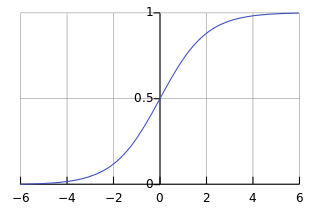
\includegraphics[width=0.27\textwidth]{images/logistic-curve.png}} \\
	{\footnotesize This squashes numbers from $(-\infty, \infty)$ to a much smaller range $(0, 1)$, with the interesting action happening around the middle}
	\pause
	\vspace{0.5em}
	\begin{codeblock}
from scipy.special import expit as logistic
logistic(2.0)  #  0.880797
	\end{codeblock}
\end{description}
\end{frame}

%\begin{frame}{Log-linear Models}
\begin{frame}[fragile]\frametitle{Log-linear Models}
	\begin{Large}
	\begin{align}
	%\hspace*{-5.5em}%
		P(y | \mathbf{x}) & = \frac{{\mathnormal e}^{\boldsymbol W_y \cdot \mathbf{x}} }{Z} \hspace*{0.4em} \substack{\color{green}{ \leftarrow \, \text{\parbox[c]{0.58\textwidth}{ {\footnotesize \, exponentiation helps ensure scores are positive}}}} \\[1.0em]  \color{green}{ \leftarrow \, \text{\parbox[c]{0.55\textwidth}{ \textbf{normalization constant}, {\footnotesize to ensure the \\[-0.9em] score of all possible outcomes sums to 1}}}}}  \nonumber\\[1.0em]
							%& = \frac{1}{Z} {\mathnormal e}^{\boldsymbol W_y \cdot \mathbf{x}}  \nonumber\\[1.0em]
							& =	\frac{{\mathnormal e}^{\boldsymbol W_y \cdot \mathbf{x}}}{\sum_h {\mathnormal e}^{\boldsymbol W_h \cdot \mathbf{x}}}  \,\, \substack{ \, \\[1.0em]  \color{green}{ \leftarrow \text{\parbox[c]{0.50\textwidth}{ \, to get Z, we just add up scores from \\[-0.8em] all possible outcomes}}}} \nonumber\\[1.0em]
							& = \text{softmax}(\boldsymbol W_y \cdot \mathbf{x}) \nonumber%\\[1.0em]
							%& =  \nonumber\\[1.0em]
	\end{align}
	\end{Large}
	\pause

	The input vector $\bf x$ includes an additional dummy value of 1.0\,, called a \textbf{bias term}.
	This helps determine the offset of the linear separator.  % (but not the shape, for nn's)
\end{frame}

\begin{frame}{Visualization}
\vspace{0.7em}
	\begin{center}
	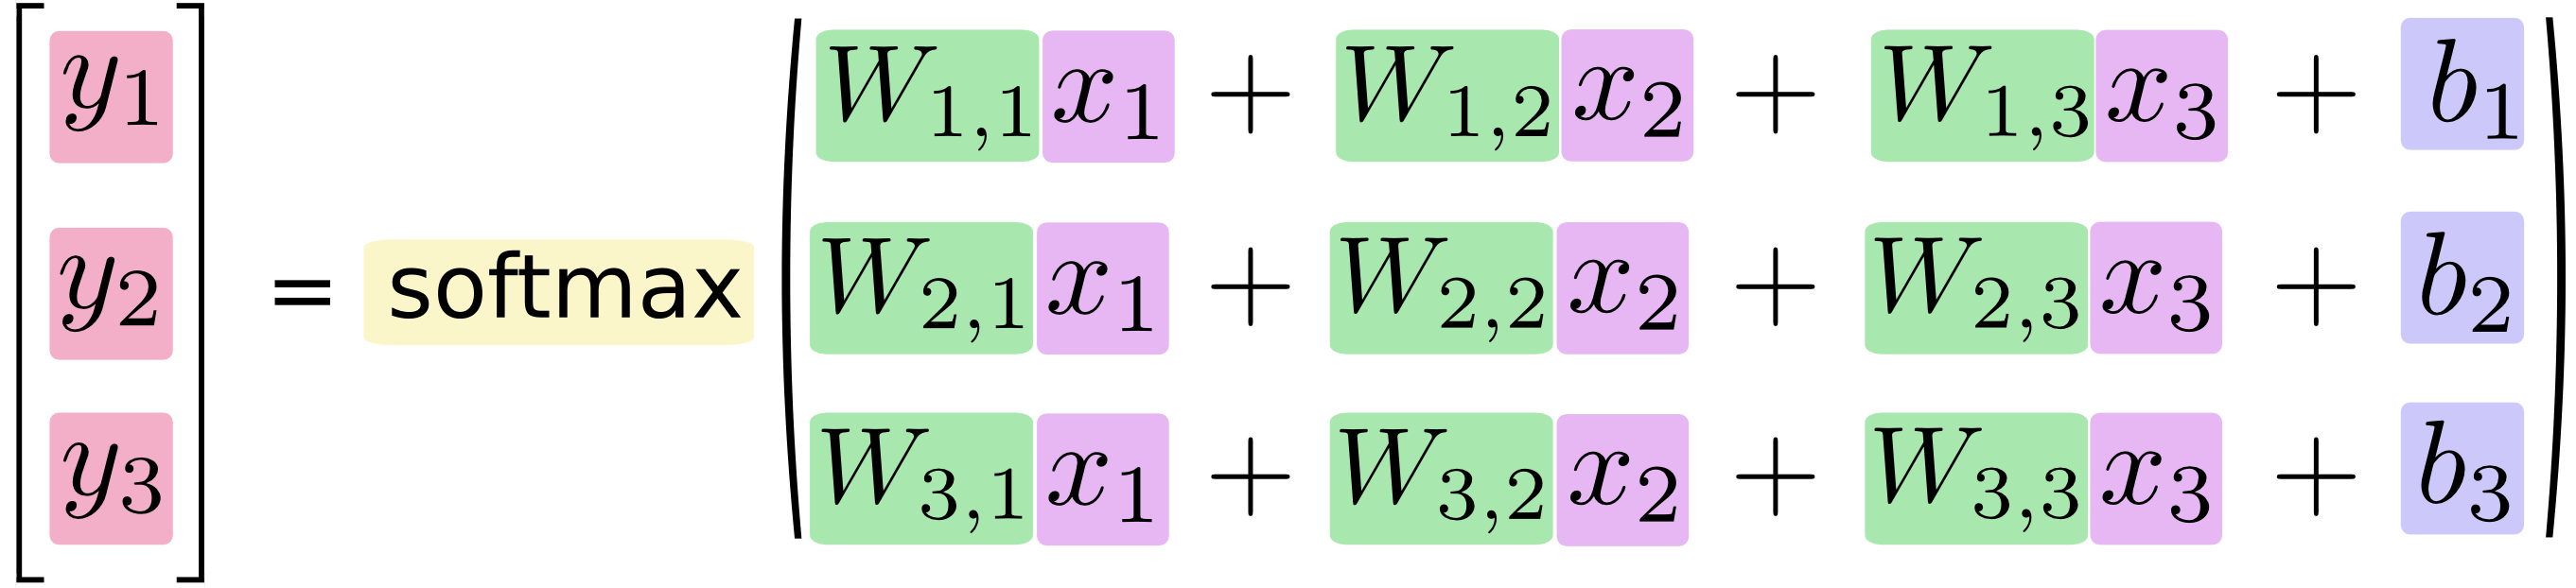
\includegraphics[height=0.19\textheight]{images/softmax-regression-scalarequation.png} \\[1.1em]
	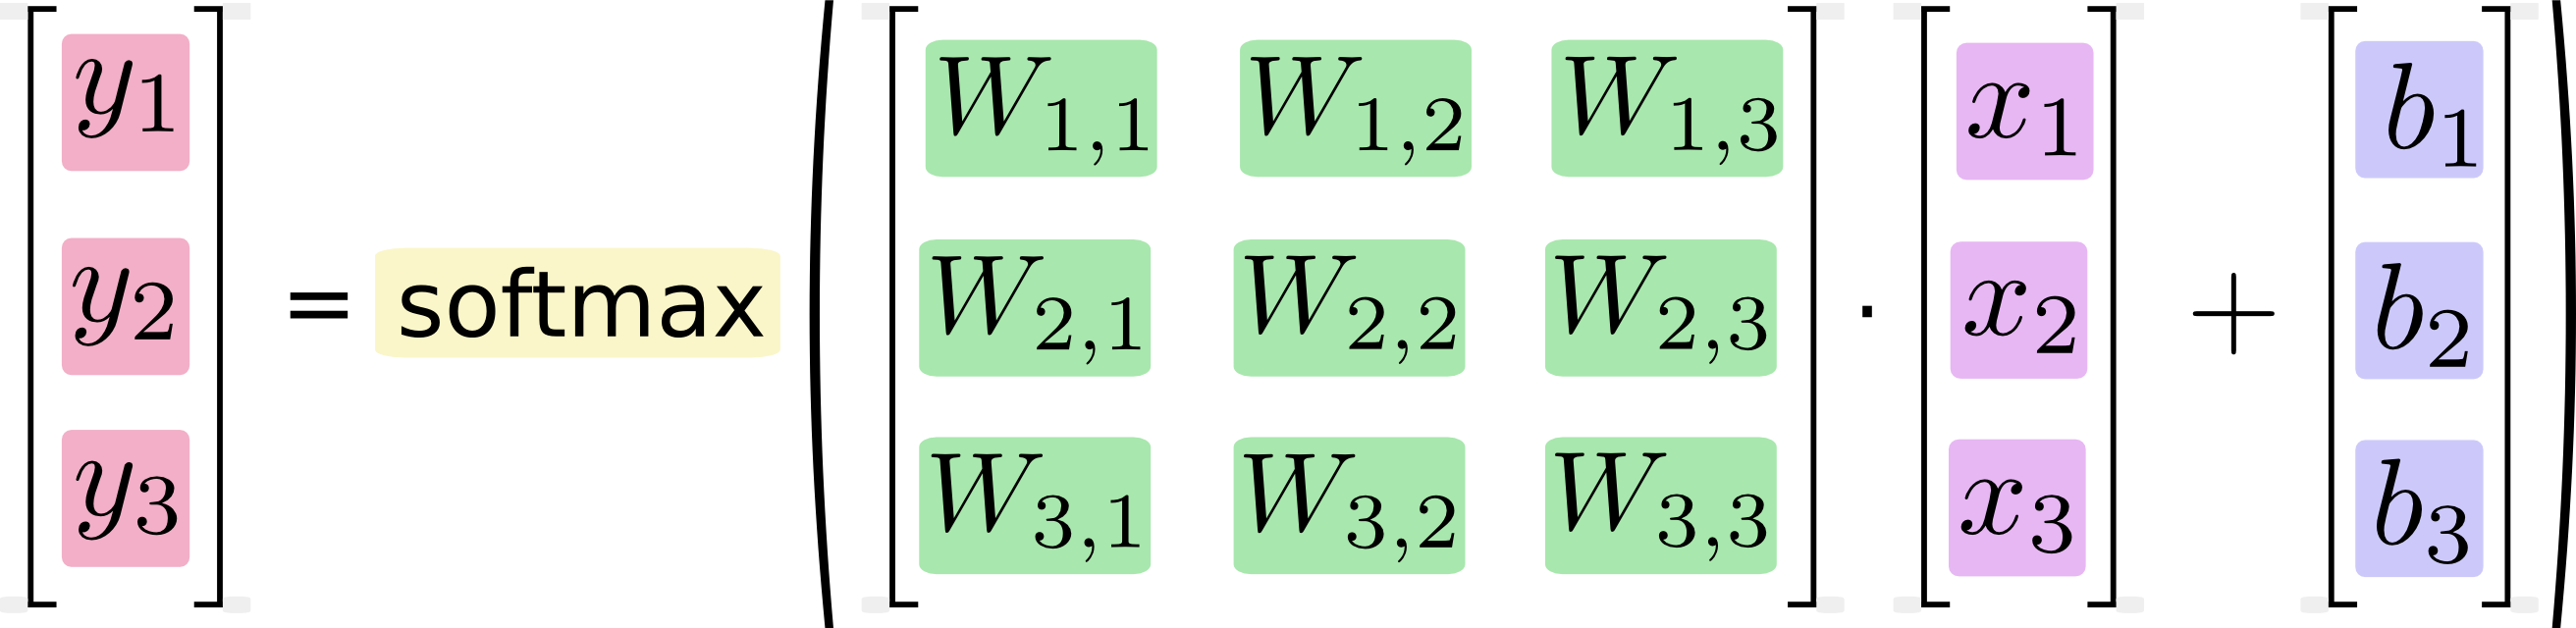
\includegraphics[height=0.19\textheight]{images/softmax-regression-vectorequation.png} \\[1.1em]
	\pause
	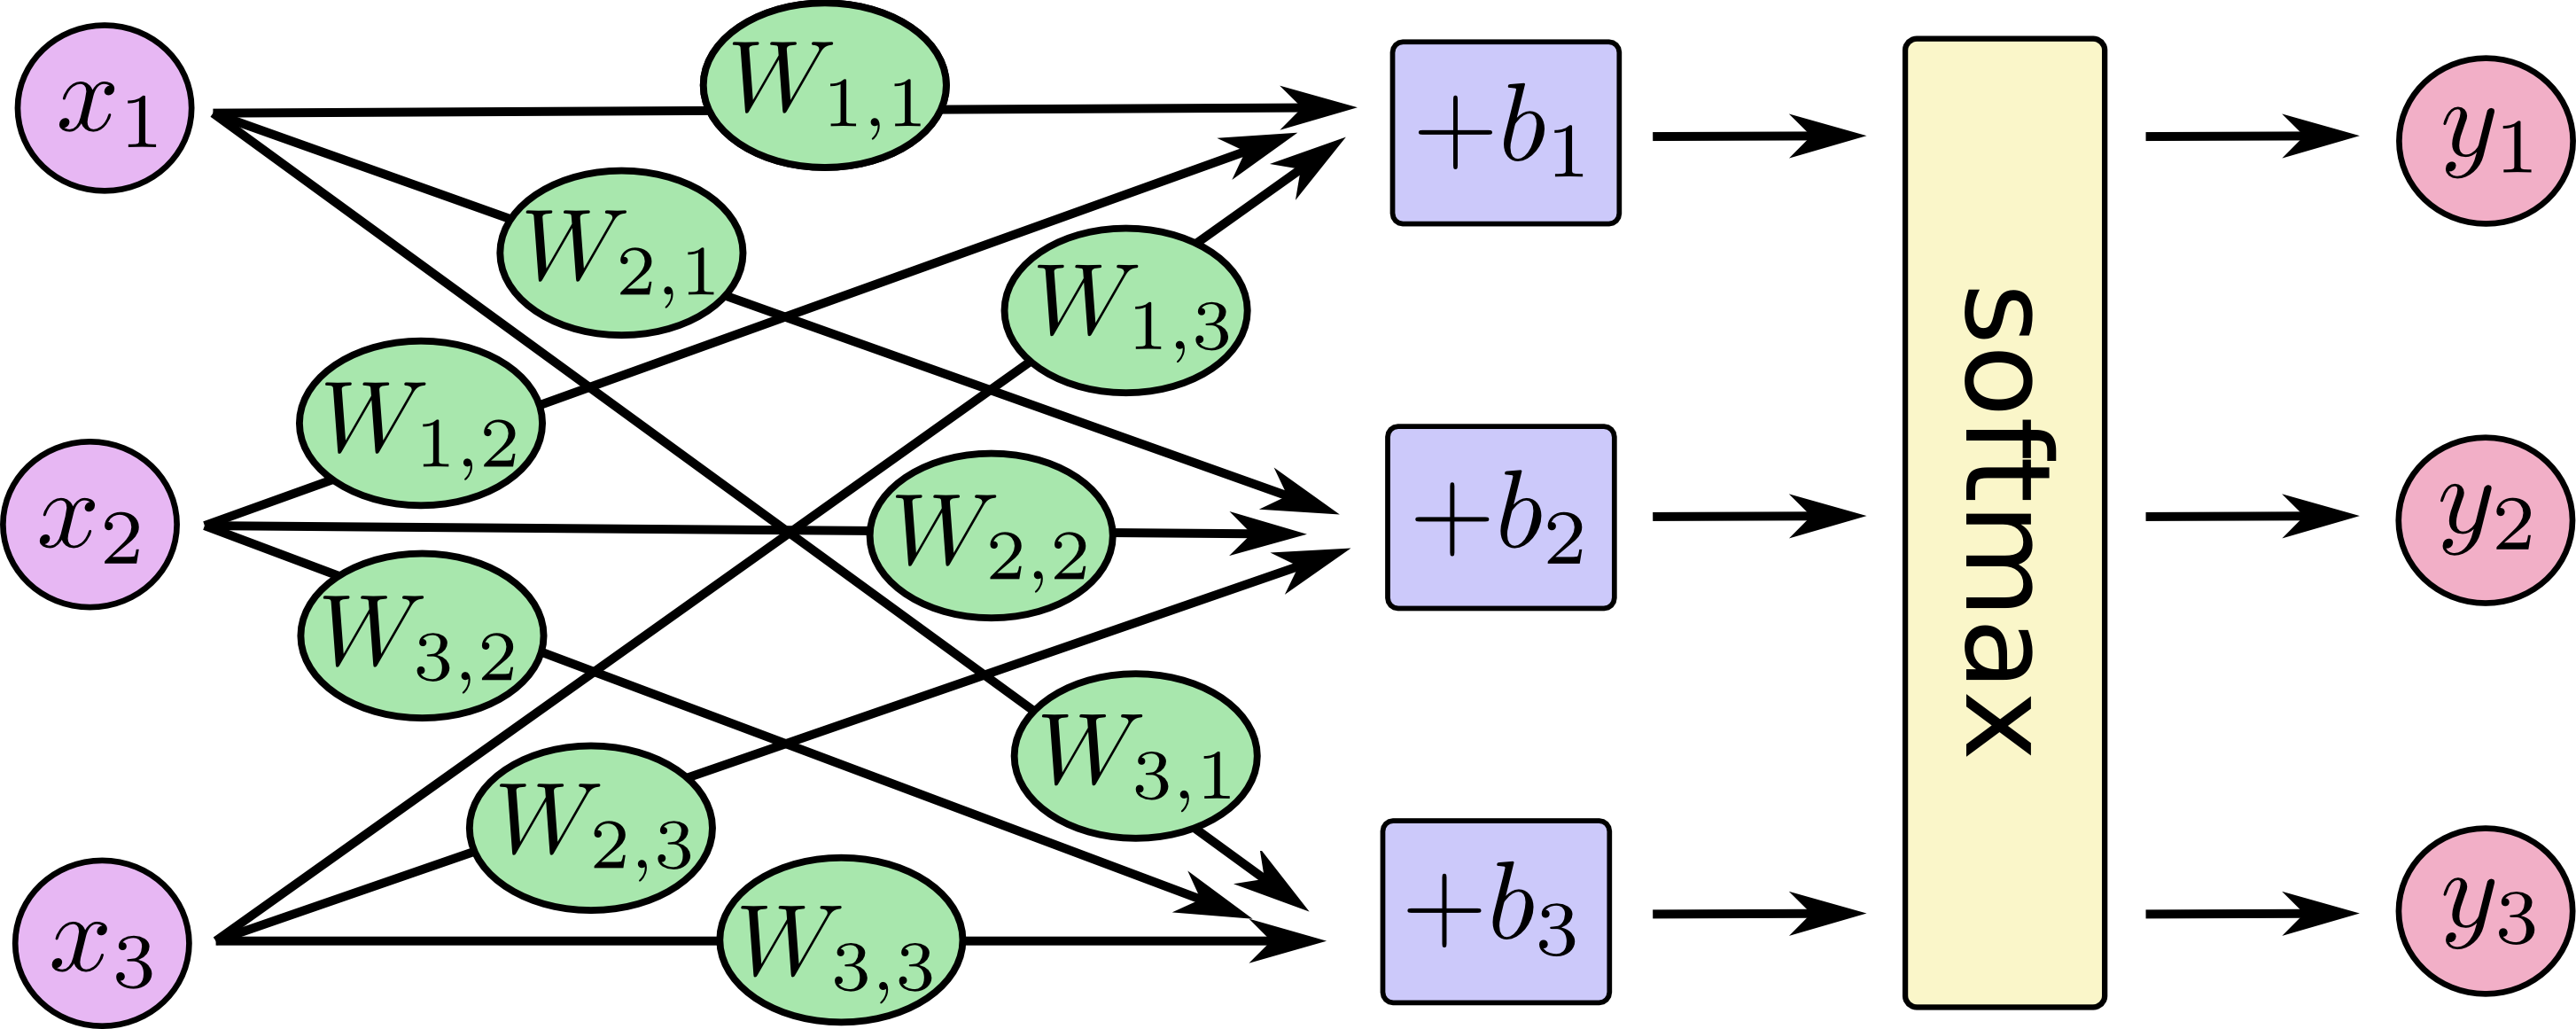
\includegraphics[height=0.29\textheight]{images/softmax-regression-scalargraph.png}
	\end{center}
\vspace{0.5em}
{\tiny Courtesy of \href{http://www.tensorflow.org/tutorials}{TensorFlow}}
\end{frame}


\begin{frame}{Finding Good Values for $\bf W$}
	\begin{center}
	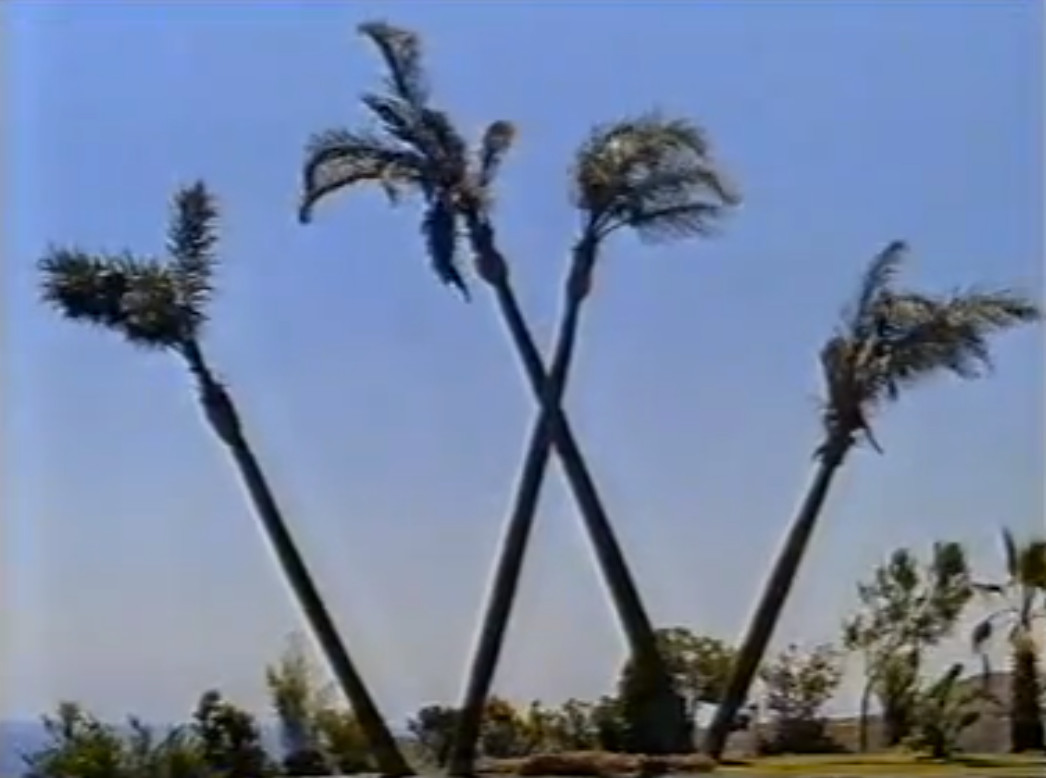
\includegraphics[width=0.36\textwidth]{images/big-w.jpg}
	\end{center}
\begin{itemize}
	\item The weight matrix $\bf W$ constitutes the \textbf{parameters} of the model
	\item Then the main task is to find good values for the weight matrix $\bf W$
	\item This is done by common \textbf{optimization} techniques, like \href{https://en.wikipedia.org/wiki/Limited-memory_BFGS}{L-BFGS} for logistic regression
\end{itemize}
\end{frame}

\begin{frame}{Terminology}
\begin{itemize}
	\item Logistic regression is over 50 years old
	\pause
	\item It's sometimes also called a \textbf{maximum entropy} classifier (MaxEnt) and softmax regression, \textit{inter alia}
	\item It also can be viewed as a \textbf{neural network} without any hidden layers
	\pause
	\item The model is called a \textbf{log-linear model}.  The following all have a log-linear model, but are trained differently:
	\begin{itemize}
		\item \textbf{Logistic regression / MaxEnt / Softmax regression}
		\item \textbf{Perceptron}
		\item \textbf{Support vector machines} (SVMs)
		\item \textbf{Conditional random fields} (CRFs)
		\item \textbf{Linear discriminant analysis} (LDA)
	\end{itemize}
\end{itemize}
\end{frame}


\begin{frame}{Perceptrons}
\begin{itemize}
	\item The perceptron is a simplified version of a biological neuron
		%\begin{center}
		\hspace*{-3.0em}%
		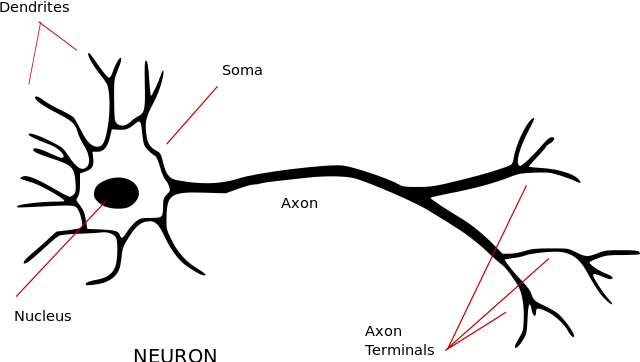
\includegraphics[width=0.42\textwidth]{images/Neuron_-_annotated.png}%
		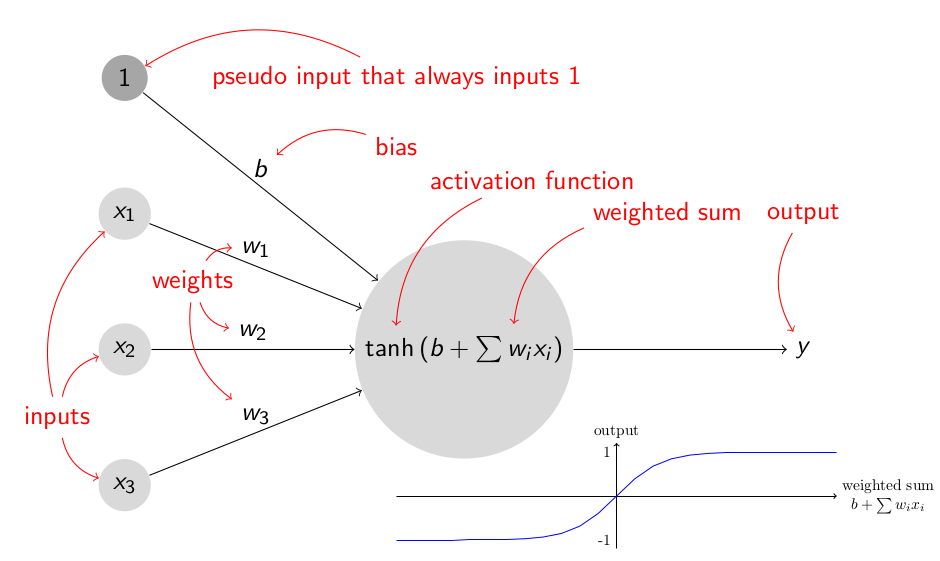
\includegraphics[width=0.62\textwidth]{images/kata_perceptron.png}
		%\end{center}
	\pause
	\item Adjusting the weights in a perceptron is really simple:
		\begin{equation*}
			w_i {\text{\tt{ +=\ }}} \eta \ \times \ \text{error} \ \times \ x_i
		\end{equation*}
	\item {\small $\bf \eta$ (`eta') is a learning rate, like 0.1, and should decrease over time } \\
	\item the \textbf{error} here is the difference between the predicted output and the correct output
\end{itemize}
{\teeny{Images courtesy of \href{https://commons.wikimedia.org/wiki/File:Neuron_-_annotated.svg}{Wikimedia} and Kata Nasz\'{a}di}}
\end{frame}


\begin{frame}{Dos Modelos}
	%\begin{tabular}{lcr}
	\begin{tabular}{>{\centering\arraybackslash}m{12em} >{\centering\arraybackslash}m{12em} }
		\Huge\bf \centering $ \frac{{\mathnormal e}^{\boldsymbol W_y \cdot \mathbf{x}} }{Z} \ \ \ \ \neq $  &  \ 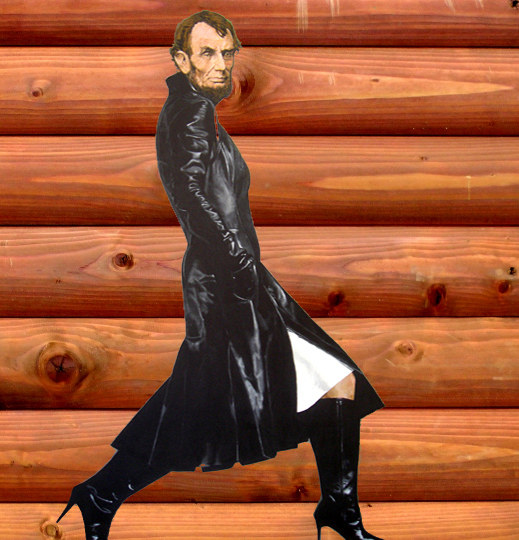
\includegraphics[width=0.5\textwidth]{images/linear-log-model.jpg} \\
		\Large\bf Log-linear Model & \Large\bf Linear-log Model \\
	\end{tabular}
\end{frame}



% \begin{frame}{}
% \begin{itemize}
% 	\item 
% 	\item 
% 	\item 
% \end{itemize}
% \end{frame}


\end{document}
